\documentclass[jou]{apa6}
\usepackage[utf8]{inputenc}
\usepackage[spanish]{babel}

\usepackage{csquotes}
\usepackage[style=apa,sortcites=true,sorting=nyt,backend=biber]{biblatex}

\usepackage{listings}

\usepackage[section]{placeins}

\DeclareLanguageMapping{spanish}{spanish-apa}
\addbibresource{bibliography.bib}

\title{HPC - Lab2: OpenMP}

\author{Rubén Cavieres Carvajal}
\affiliation{Universidad de Santiago de Chile}

\leftheader{DIINF-USACH}

\abstract{Se presenta un resumen del desarrollo del laboratorio 2 de la asignatura High Performance Computing dictado por el profesor Dr. Fernando Rannou, exponiendo resultados de las pruebas de rendimiento computacional sobre la aplicación paralelizada.}

\keywords{HPC, OpenMP, Parallel, Schroedinger}

\begin{document}
\maketitle
El trabajo comienza con la creación de un algoritmo secuencial que simula el comportamiento de una onda bajo la ley de Schroedinger.

Luego se identifican las piezas de código que pueden ser paralelizables para utilizar en éstas estrategias basadas en OpenMP.

Finalmente se realizan pruebas de rendimiento de la aplicación utilizando las métricas:

\begin{itemize}
	\item Tiempo de ejecución (wall-clock)
	\item Speedup relativo
	\item Eficiencia
\end{itemize}


\section{Algoritmo}
\subsection{Ecuaciones}
El algoritmo se estructuró de tal forma que represente el planteamiento del matemático. Es decir, consideró las condiciones de la variable tiempo $t$ para utilizar las ecuaciones con los siguientes métodos:

\begin{itemize}
	\item \texttt{initializeSpace}: Para $t = 0$ inicializa el espacio (grilla) de trabajo, dado por el impulso en celdas centrales en grilla.
	\item \texttt{fillSpaceFirstStep}: Para $t = 1$ genera la primera iteración de la onda utilizando $H^{t-1}$.
	\item \texttt{fillSpaceTSteps}: Para $t > 1$ genera las sucesivas iteraciones de la onda, utilizando los estados del espacio $H^{t-1}$ y $H^{t-2}$.
\end{itemize}

\subsection{Paralelización}
La estrategia de paralelización se basó en decubrir los bloques de códigos críticos potenciales para la utilización de OpenMP.

Estos trozos de código fueron las ecuaciones de Schroedinger para el intervalo de tiempo $t >= 1$:

\lstset{language=C, breaklines=true, frame=single}

\begin{lstlisting}
#pragma omp parallel num_threads(H)
#pragma omp for schedule(static, 4)
for (int i = 1; i < N; i++)
for (int j = 1; j < N - 1; j++)
	waveSpace[N * i + j] = 2 * waveSpaceTMin1[N * i + j] - waveSpaceTMin2[N * i + j] + (c * c) * (dt/dd * dt/dd) * (waveSpaceTMin1[N * (i + 1) + j] + waveSpaceTMin1[N * (i - 1) + j] + waveSpaceTMin1[N * i + (j - 1)] + waveSpaceTMin1[N * i + (j + 1)] - 4 * waveSpaceTMin1[N * i + j]);
\end{lstlisting}

Como se aprecia en código de instrucción \texttt{parallel for}, debido al empleo de 4 celdas que realiza la ecuación de Schroedinger, es que se decidió utilizar una paralelización estática asignando a cada hilo una cantidad fija de 4 iteraciones del bucle. 

\section{Rendimiento Computacional}

El análisis de rendimiento se realizó bajo los siguientes parámetros y valores:

\begin{itemize}
	\item hebras = \{1, 2, 3, ..., 14\}
	\item grillas = \{128, 256\}
	\item pasos = \{2000, 4000, 8000\}
\end{itemize}

Los tamaños de imagen considerados para el estudio son de 128 y 256 pixeles.

\subsection{Tiempo}

\subsubsection{N = 128}
El tiempo tomado para realizar la ejecución se representa en la siguiente figura:

\clearpage

\begin{figure}[h]
	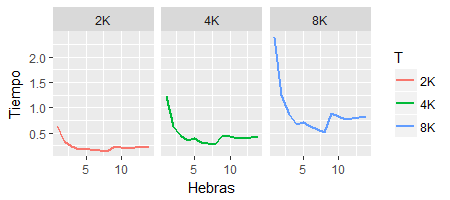
\includegraphics[width=\columnwidth]{tiempo-128px.png}
	\caption{Tiempo ejecución para T = \{2000, 4000, 8000\}}
	\label{fig:Figure1}
\end{figure}

Se observa que hay una suave caída en el tiempo a medida que aumenta el número de hilos, llegando a los siguientes mínimos: 

% Please add the following required packages to your document preamble:
% \usepackage{booktabs}
\begin{table}[h]
\centering
\caption{Mínimos de tiempo por iteraciones.}
\label{my-label}
\begin{tabular}{@{}lll@{}}
\toprule
\multicolumn{1}{c}{T (its.)} & \multicolumn{1}{c}{H (num.)} & \multicolumn{1}{c}{T (seg.)} \\ \midrule
2000                         & 8                            & 0,142299                     \\
4000                         & 6                            & 0,267584                     \\
8000                         & 8                            & 0,503911                     \\ \bottomrule
\end{tabular}
\end{table}

A partir de estos mínimos, tiempo se estabiliza, sin haber mayores cambios hasta la última iteración.

\subsubsection{N = 256}
Aumentando el tamaño de grilla, se descubre lo siguiente:

\begin{figure}[h]
	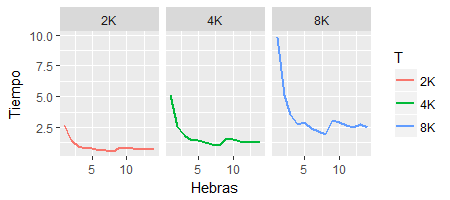
\includegraphics[width=\columnwidth]{tiempo-256px.png}
	\caption{Tiempo ejecución para T = \{2000, 4000, 8000\}}
	\label{fig:Figure2}
\end{figure}


El comportamiento de la curva en comparación al anterior es equivalente, registrando los siguientes mínimos:

\begin{table}[h]
\centering
\caption{Mínimos de tiempo por iteraciones.}
\label{my-label}
\begin{tabular}{@{}lll@{}}
\toprule
\multicolumn{1}{c}{T (its.)} & \multicolumn{1}{c}{H (num.)} & \multicolumn{1}{c}{T (seg.)} \\ \midrule
2000                         & 8                            & 0,569594                     \\
4000                         & 8                            & 1,036259                     \\
8000                         & 8                            & 1,899529                     \\ \bottomrule
\end{tabular}
\end{table}

Hay tan solo un aumento en el tiempo mínimo por la particularidad de estar trabajando sobre una grilla de mayor dimensión.

\FloatBarrier

\subsection{Speedup}
La métrica utilizada para calcular el \textit{speedup} fue el relativo, el cual se expresa de la siguiente forma:

\[
	S_{relativo}(I, H) = \frac{tiempo\, resolv.\, I\, usando\, programa\, Q\, y\, 1\, hebra}{tiempo\, resolv.\, I\, usando\, programa\, Q\, y\, H\, hebras}
\]

\subsubsection{N = 128}
El resultado del análisis de rendimiento arroja lo siguiente:

\begin{figure}[h]
	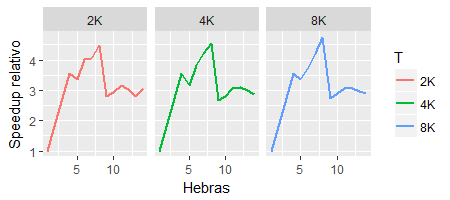
\includegraphics[width=\columnwidth]{srel-128px.png}
	\caption{Speedup relativo para T = \{2000, 4000, 8000\}}
	\label{fig:Figure3}
\end{figure}

Para los tres pasos analizados, se observa un notorio incremento hasta alrededor de la ejecución con 8 hebras, a partir de donde se precipita hasta cerca de la hebra 10, manteniendo sucesivamente un valor constante.

Los máximos para cada paso son:

\begin{table}[h]
\centering
\caption{Máximo de speedup por iteraciones}
\label{my-label}
\begin{tabular}{@{}lll@{}}
\toprule
\multicolumn{1}{c}{T (its.)} & \multicolumn{1}{c}{H (num.)} & \multicolumn{1}{c}{T (seg.)} \\ \midrule
2000                         & 8                            & 4,4754847                    \\
4000                         & 8                            & 4,5470394                    \\
8000                         & 8                            & 4,7375529                    \\ \bottomrule
\end{tabular}
\end{table}

\clearpage

\subsubsection{N = 256}
Mismo análisis con tamaño de grilla incrementado produce sutilmente mejores resultados, donde la curva en toda su prolongación tiene un pequeño incremento.

\begin{figure}[h]
	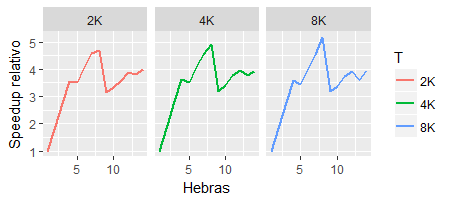
\includegraphics[width=\columnwidth]{srel-256px.png}
	\caption{Speedup relativo para T = \{2000, 4000, 8000\}}
	\label{fig:Figure4}
\end{figure}

Junto con lo anterior, la tendencia de la curva es similar a aquella obtenida con el tamaño de grilla menor.

Sus máximos para cada paso son los siguientes:

\begin{table}[h]
\centering
\caption{Máximo de speedup por iteraciones}
\label{my-label}
\begin{tabular}{@{}lll@{}}
\toprule
\multicolumn{1}{c}{T (its.)} & \multicolumn{1}{c}{H (num.)} & \multicolumn{1}{c}{T (seg.)} \\ \midrule
2000                         & 8                            & 4,7063189                    \\
4000                         & 8                            & 4,9117817                    \\
8000                         & 8                            & 5,1620396                    \\ \bottomrule
\end{tabular}
\end{table}

\FloatBarrier

\subsection{Eficiencia}
La eficiencia fue calculada por medio la siguiente ecuación:

\[
	E(H) = \frac{S_{relativo}(I, 1)}{S_{relativo}(I, H) * H}
\]

Los resultados arrojados por el cálculo de la eficiencia son los siguientes:

\subsubsection{N = 128}
Mismo análisis con tamaño de grilla incrementado produce:

\begin{figure}[h]
	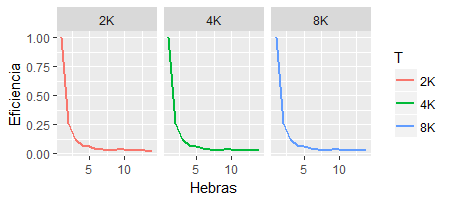
\includegraphics[width=\columnwidth]{efic-128px.png}
	\caption{Eficiencia para T = \{2000, 4000, 8000\}}
	\label{fig:Figure5}
\end{figure}

Hay un decremento sostenido del indicador hasta la ejecución con 3 hebras, desde donde curva se estabiliza.

El punto de inflexión dado con \textit{H = 3} para cada iteración tiene el siguiente valor:

\begin{table}[]
\centering
\caption{Punto inflexión eficiencia por iteraciones}
\label{my-label}
\begin{tabular}{@{}lll@{}}
\toprule
\multicolumn{1}{c}{T (its.)} & \multicolumn{1}{c}{H (num.)} & \multicolumn{1}{c}{E(H)} \\ \midrule
2000                         & 3                            & 0,3718947                \\
4000                         & 3                            & 0,3491872                \\
8000                         & 3                            & 0,352224                 \\ \bottomrule
\end{tabular}
\end{table}

\subsubsection{N = 256}
Mismo análisis con tamaño de grilla incrementado produce los resultados expresados en grilla.

\begin{figure}[h]
	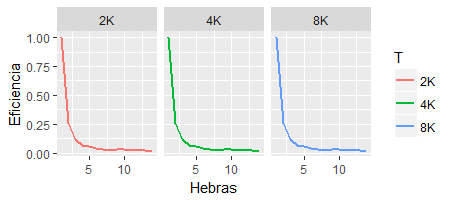
\includegraphics[width=\columnwidth]{efic-256px.png}
	\caption{Eficiencia para T = \{2000, 4000, 8000\}}
	\label{fig:Figure6}
\end{figure}

La curva se comporta de manera similar al numero de pasos anterior, con sus respectivos valores en la curva de inflexión:

\begin{table}[h]
\centering
\caption{Punto inflexión eficiencia por iteraciones}
\label{my-label}
\begin{tabular}{@{}lll@{}}
\toprule
\multicolumn{1}{c}{T (its.)} & \multicolumn{1}{c}{H (num.)} & \multicolumn{1}{c}{E(H)} \\ \midrule
2000                         & 3                            & 0,4842093                \\
4000                         & 3                            & 0,4627912                \\
8000                         & 3                            & 0,4759161                \\ \bottomrule
\end{tabular}
\end{table}

\section{Conclusiones}
A partir de la comparación de los resultados para cada variación de parámetro del algoritmo, se observa que las curvas de tiempo, \textit{speedup} y eficiencia se presentan similares, evidenciando que la estrategia de paralelización aplicada fue estática. 

Esta característica de paralelización garantizó que el trabajo con hilos se realizara uniformemente dentro del bucle de construcción de grilla con imagen.

Un inconveniente en el análisis de rendimiento fue que se contó con un computador de 8 núcleos, cuya característica no permitió extender el análisis con una mayor cantidad de cómputo que permitiera ver el comportamiento de la aplicación en un periodo de tiempo más extenso.

\end{document}
